\section{Grothendieck Ineqaulity}

\begin{frame}
	\begin{lemma}[Grothendieck's identity]\label{lem:G_id}
		Let $x,y\in\mathbb{R}^d$ be unit vectors. Let $r\in\mathbb{R}^d$ be a random unit vector chosen from $O(d)$-invariant probability distribution on the unit sphere. Then
		\begin{enumerate}
			\item[i,] $\mathbb{P}[\sgn(\sclr{x}{r})\neq\sgn(\sclr{y}{r})]=\frac{\arccos(\sclr{x}{y})}{\pi}$
			\item[ii,] $\mathbb{E}[\sgn(\sclr{x}{r})\sgn(\sclr{y}{r})]=\frac{2}{\pi}\arcsin(\sclr{x}{y}).$
		\end{enumerate}
	\end{lemma}
	\begin{pbmr}
		\begin{itemize}
			\item<1-> if $x$ and $y$ are linearly dependent, then
				\begin{itemize}
					\item<2-> if $x=y$:~~\, $\arccos(\sclr{x}{y})=\arccos(1) = 0$
					\item<3-> if $x=-y$: $\arccos(\sclr{x}{y})=\arccos(-1) = \pi$
				\end{itemize}
			\item<4-> if $x$ and $y$ are linearly independent, then 
				\begin{itemize}
					\item<5-> project $r$ orthogonally on $\spn\{x,y\}$ which gives us a vector $s$ with $\sclr{x}{r} = \sclr{x}{s}$ and $\sclr{y}{r} = \sclr{y}{s}$
					\item<6-> the normalized vector $n\coloneqq s/\norm{s}$ is uniformly distributed on the intersection of the unit sphere and $\spn\{x,y\}$ by the $O(d)$-invariance of the probability distribution
				\end{itemize}
		\end{itemize}
	\end{pbmr}
\end{frame}

\begin{frame}
	\begin{pbmr}
		\begin{figure}
			\begin{center}
				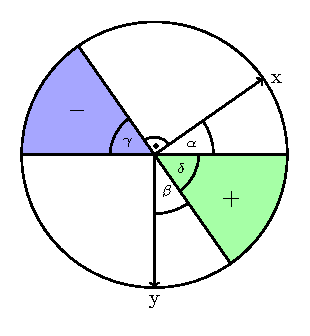
\includegraphics[width=0.38\textwidth]{ChapersPresentation/fig_unit_circle.pdf}
			\end{center}
		\end{figure}
	\end{pbmr}
\end{frame}